\documentclass[12pt]{article}
% \documentclass[answers]{exam}

%Formatting Libraries
\usepackage[english]{babel}
\usepackage[utf8]{inputenc}
\usepackage[autostyle, english = american]{csquotes}
\MakeOuterQuote{"}
\usepackage{listings}
\usepackage{keyval}
\usepackage{xcolor}
\usepackage{textcomp}
\usepackage{fullpage}
\usepackage{setspace}
\usepackage{graphicx}
\usepackage{hyperref}
\usepackage{verbatim}
%\usepackage[]{mcode}
\usepackage{multicol}
\usepackage{float}
\usepackage{framed}
\usepackage{parskip}
\setlength{\parindent}{15pt}
\usepackage[fleqn]{amsmath}
\usepackage{pifont}% http://ctan.org/pkg/pifont
\newcommand{\cmark}{\ding{51}}%
\newcommand{\xmark}{\ding{55}}%
\usepackage{cancel}
\usepackage{algorithm2e} % algorithm package
\usepackage{tcolorbox} % wrap box around solution or something
\usepackage{mdframed} % frame solutions
\usepackage{lipsum}

%Symbols Libraries
\usepackage[fleqn]{amsmath}
\usepackage{amssymb}
\usepackage{amsfonts}
\usepackage{amsthm}
\usepackage{marvosym}
\usepackage{wasysym}
\usepackage{slashbox}

%For Image Generation
\usepackage{tikz}
\usepackage{tkz-euclide}
\usetikzlibrary{positioning}
\usetikzlibrary{arrows}
\usepackage[toc,page]{appendix}  % Appendix package

%For Theorem Environment
\newtheorem{theorem}{Theorem}
%Theorems numbering follow section numbers
\newtheorem{definition}[theorem]{Definition}
%definitions follow the number system that theorems do
\newtheorem{lemma}[theorem]{Lemma}
\newtheorem{corollary}[theorem]{Corollary}
\newtheorem{remark}[theorem]{Remark}
\newtheorem{proposition}[theorem]{Proposition}
%lemmas & corollaries follow the same number system as theorems do

%Making shortcuts
\renewcommand\qedsymbol{$\blacksquare$}
\newcommand{\rup}[1]{\overset{\rightharpoonup}{#1}}
\newcommand{\C}{\mathbb C}
\newcommand{\Q}{\mathbb Q}
\newcommand{\F}{\mathbb F}
\newcommand{\R}{\mathbb R}
\newcommand{\Z}{\mathbb Z}
\newcommand{\N}{\mathbb N}
\newcommand{\rank}[1]{\mathrm{rank}\left({}#1\right)}
\newcommand{\ran}[1]{\text{Ran}\left({}#1\right)}
\newcommand{\diag}[1]{\text{diag}\left({}#1\right)}
\newcommand{\nullity}{\mathrm{nullity}}
\newcommand{\st}{ \ |\ }
\newcommand{\DS}{\displaystyle}
\newcommand{\RA}{\Rightarrow}
\newcommand{\LA}{\Leftarrow}
\newcommand{\LRA}{\Leftrightarrow}
\newcommand{\ip}[2]{\left\langle{}#1,#2\right\rangle{}}
\newcommand{\lip}[2]{\left({}#1,#2\right){}}
\renewcommand{\labelenumii}{\alph{enumii}.)}
\newcommand{\curly}[1]{\left\{{}#1\right\}}
\newcommand{\eps}{\varepsilon}
\newcommand{\emp}{\varnothing}
\newcommand{\ellinf}{\ell^{\infty}}
\newcommand{\inv}{^{-1}}
\newcommand{\sgn}{\text{sgn}}
\newcommand{\tr}[1]{\text{tr}\left({}#1\right)}
\newcommand{\norm}[1]{\left|\left|{}#1\right|\right|}
\newcommand{\infnorm}[1]{\left|\left|{}#1\right|\right|_{\infty}}
\newcommand{\linfnorm}[1]{\left|\left|{}#1\right|\right|_{L^{\infty}}}
\newcommand{\onenorm}[1]{\left|\left|{}#1\right|\right|_1}
\newcommand{\twonorm}[1]{\left|\left|{}#1\right|\right|_2}
\newcommand{\xnorm}[1]{\left|\left|{}#1\right|\right|_X}
\newcommand{\abs}[1]{\left|{}#1\right|}
\newcommand{\pare}[1]{\left({}#1\right)}
\newcommand{\brak}[1]{\left[{}#1\right]}
\newcommand{\red}[1]{\textcolor{red}{#1}}
\newcommand{\green}[1]{\textcolor{Green}{#1}}
\newcommand{\floor}[1]{\lfloor #1 \rfloor}
\newcommand{\ceil}[1]{\lceil #1 \rceil}
\newcommand{\tif}{\text{ if }}
\newcommand{\ve}[1]{\textbf{#1}}
\newcommand{\St}{\text{S.t. }}
\newcommand{\bmat}[1]{\begin{bmatrix} #1 \end{bmatrix}}
\newcommand{\pmat}[1]{\begin{pmatrix} #1 \end{pmatrix}}
\newcommand{\spn}{\text{span}}
\newcommand{\aut}[1]{\text{Aut}\left({}#1\right)}
\newcommand{\inn}[1]{\text{Inn}\left({}#1\right)}
\newcommand{\var}[1]{\text{Var}\left({}#1\right)}
\newcommand{\cond}[1]{\text{cond}\left({}#1\right)}
\newcommand{\cov}[2]{\text{Cov}\left({}#1,#2\right){}}
\newcommand{\divergence}{\nabla \cdot}
\newcommand{\curl}{\nabla \times}
\newcommand{\omint}{\int_{\Omega}}
\newcommand{\tsp}{\vspace{3mm}}
\newcommand{\ul}[1]{\underline{#1}}

% brackets on the right
\newenvironment{rcases}
  {\left.\begin{aligned}}
  {\end{aligned}\right\rbrace}

%To make it so that the equation number follows subsections
\numberwithin{equation}{section}

% ¯\_(ツ)_/¯
\newcommand{\shrug}[1][]{%
\begin{tikzpicture}[baseline,x=0.8\ht\strutbox,y=0.8\ht\strutbox,line width=0.125ex,#1]
\def\arm{(-2.5,0.95) to (-2,0.95) (-1.9,1) to (-1.5,0) (-1.35,0) to (-0.8,0)};
\draw \arm;
\draw[xscale=-1] \arm;
\def\headpart{(0.6,0) arc[start angle=-40, end angle=40,x radius=0.6,y radius=0.8]};
\draw \headpart;
\draw[xscale=-1] \headpart;
\def\eye{(-0.075,0.15) .. controls (0.02,0) .. (0.075,-0.15)};
\draw[shift={(-0.3,0.8)}] \eye;
\draw[shift={(0,0.85)}] \eye;
% draw mouth
\draw (-0.1,0.2) to [out=15,in=-100] (0.4,0.95); 
\end{tikzpicture}}

\begin{document}
\begin{center}
\begin{large}
Math 9830\\
Final Write-Up\\
Sean Ingimarson
\end{large}
\end{center}

\section{Introduction and Background Information}

Simulating turbulent flow has been a major field of research for the last several decades.  We model this using the unsteady Navier-Stokes equation given below:
\begin{align}
u_t-\nu \Delta u+u \cdot \nabla u + \nabla p &= f, \label{eq:NS1}\\
\divergence u&=0, \label{eq:NS2}
\end{align}
where $u$ is the vector valued function modeling velocity, $p$ is a scalar function modeling pressure, and $\nu$ is viscosity.  Using finite element on \eqref{eq:NS1}-\eqref{eq:NS2} brings about issues because of the nonlinear term $u \cdot \nabla u$.

To maintain a physically relevant formulation, we would like our weak form to conserve various important physical quantities, namely energy, momentum, and angular momentum.  It is shown in \cite{CHOR17} that the base formulation does not conserve these quantities, hence is not the most desirable formulation.  The EMAC (energy, momentum, and angular momentum conserving) formulation does however conserve these quantities and more.  The strong form is defined as
\begin{align}
u_t-\nu \Delta u + 2D(u)u+(\divergence u)u+ \nabla p &= f, \label{eq:emac1}\\
\divergence u&=0. \label{eq:emac2}
\end{align}
$D$ is the symmetric gradient, also note that \eqref{eq:emac1} is mathematically equivalent to \eqref{eq:NS1} using \eqref{eq:NS2}.  However discretely, this is not always the case, which causes issues in implementation.

To further strengthen the EMAC scheme, we would like to introduce a spatial filter to the nonlinear term.  Namely
\begin{align}
u_t-\nu \Delta u + 2D(w)w+(\divergence w)w+ \nabla p &= f, \label{eq:emacreg1}\\
-\alpha^2 \Delta w + w & = u, \label{eq:emacreg2}\\
\divergence u&=0. \label{eq:emacreg3}
\end{align}
We call this formulation EMAC-Reg (energy, momentum, angular momentum conserving regularization).  We show in \cite{I20} that this formulation does indeed preserve energy, momentum, and angular momentum.  We also show numerical results that show that EMAC-Reg performs better on a coarser mesh.

Performing well on a coarse mesh is advantageous for a multitude of reasons.  Computing 3D turbulence problems can give us millions of DoFs, which is very expensive.  Having a more accurate solution on a less refined mesh will save tons of computation time.

\section{Goal and Expectations}

The goal of this project is utilize EMAC-Reg in deal.ii and be able to perform 3d problems.  This however didn't hapen due to time (and intelligence) constraints, but implementing EMAC was more feasible and was achieved.  We also would like to compute energy, momentum and angular momentum at every timestep and compare it with previous results.

Also creating a benchmark problem to confirm convergence rates was also on the schedule, which unfortunately also wasn't feasible in the time that was left.

Below are some figures that we expect to see.  We have a reference plot along with different formulations on a coarse mesh.
\begin{figure}[H]
\centering
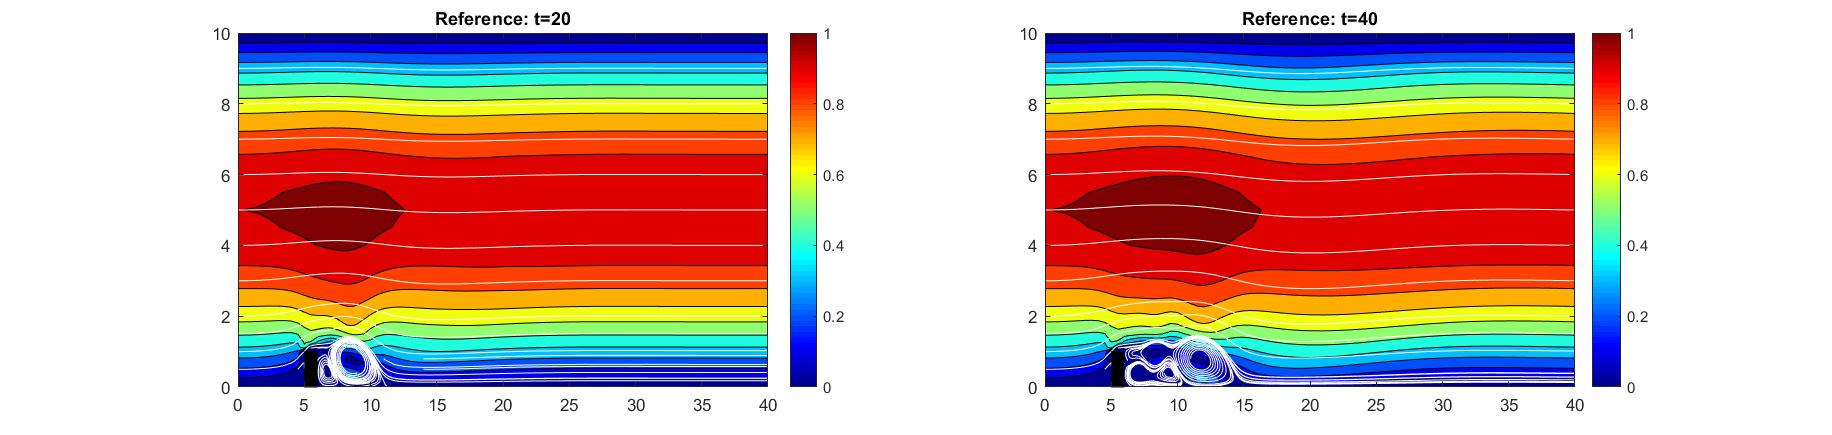
\includegraphics[scale=.25]{step_Skew_fine.jpg}
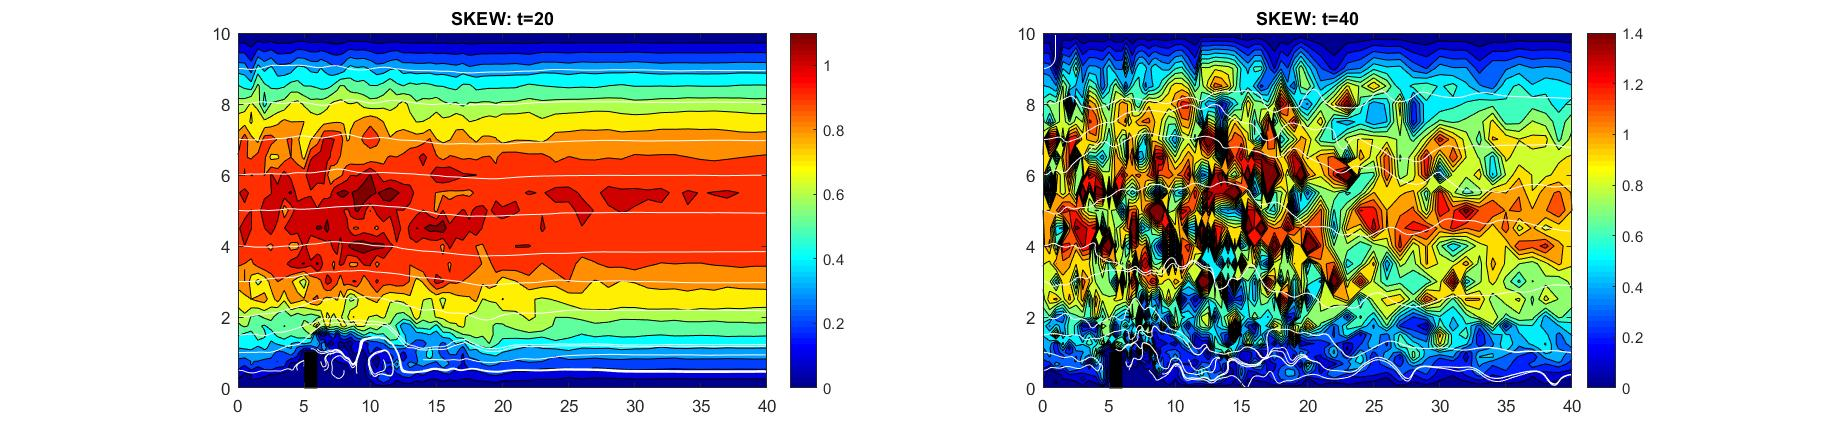
\includegraphics[scale=.25]{step_skew_coarse.jpg}
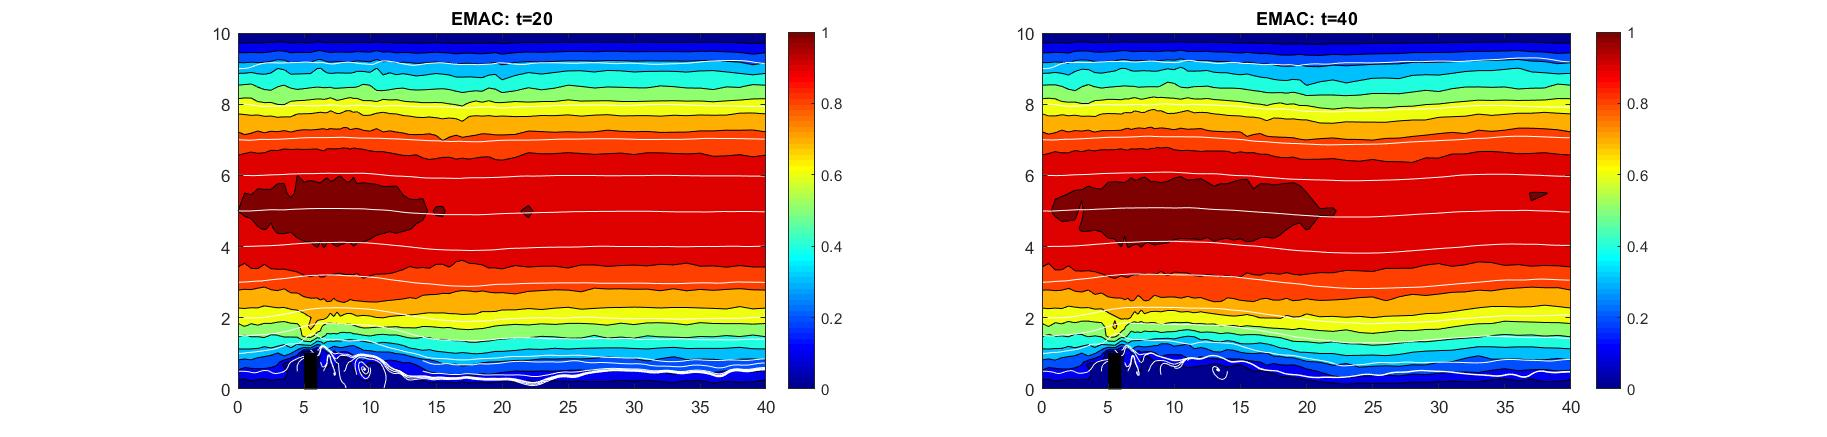
\includegraphics[scale=.25]{step_EMAC_coarse.jpg}
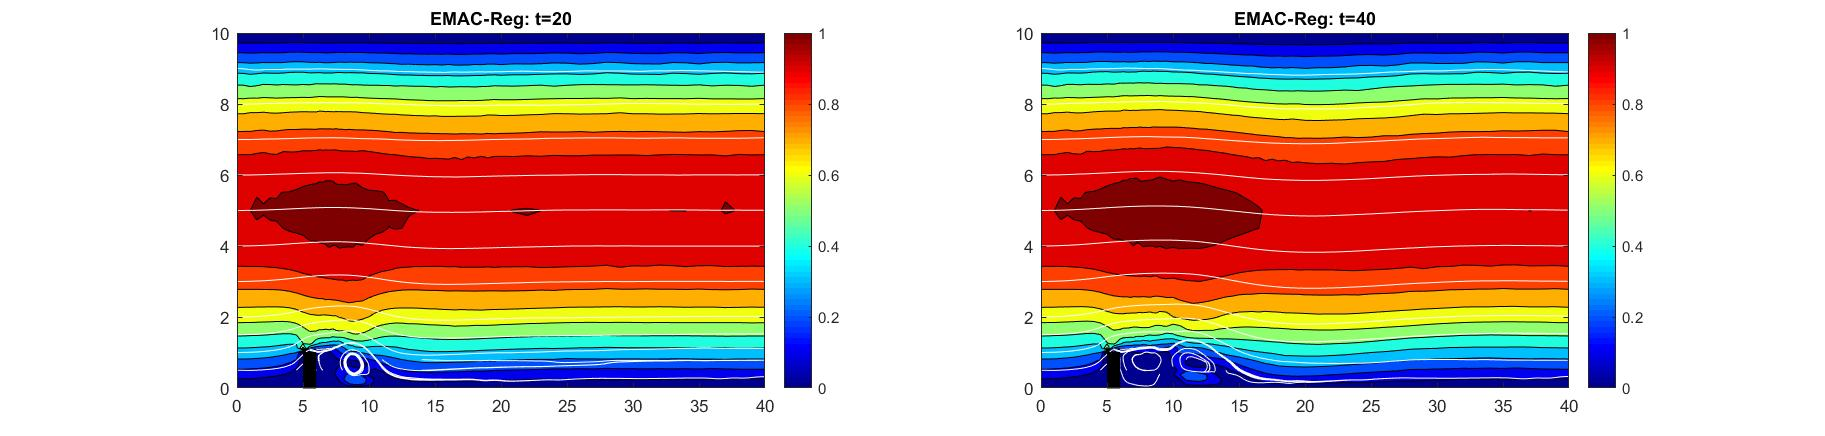
\includegraphics[scale=.25]{step_EMAC_Reg_coarse.jpg}
\end{figure}

These tables show the strength of EMAC-Reg over other formulations, that being said EMAC still performs well, so we should expect to see good results.

Below are results from \cite{I20} which show how these formulations compare for the quantities discussed.

\begin{figure}[H]
\centering
\includegraphics[scale=.4]{Quant_comparison.jpg}
\end{figure}

\section{Results}

The main result from this project was turbulent flow past a channel with a cylinder.  Below are some screenshots and attached will be the video file at times $t=2,2.5,3,3.5$.

\begin{figure}[H]
\centering
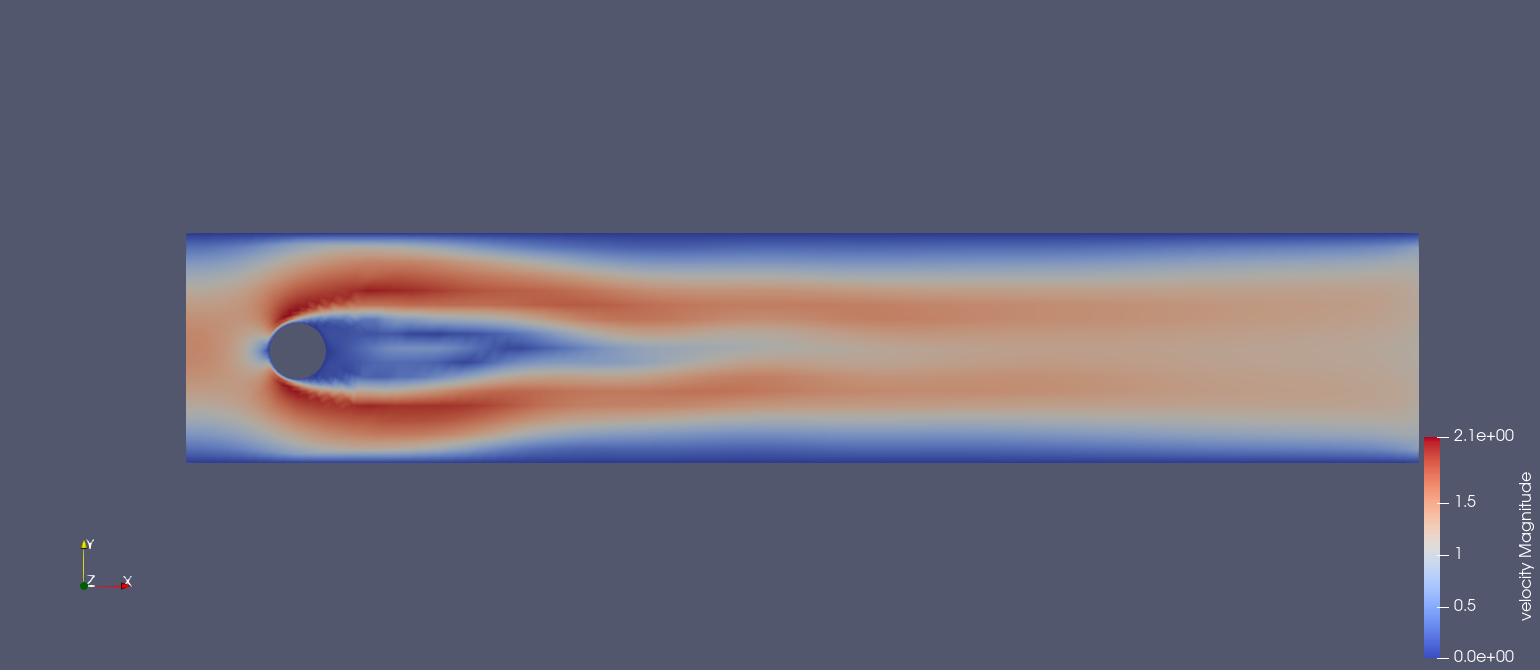
\includegraphics[scale=.2]{EMAC_time_2.png}
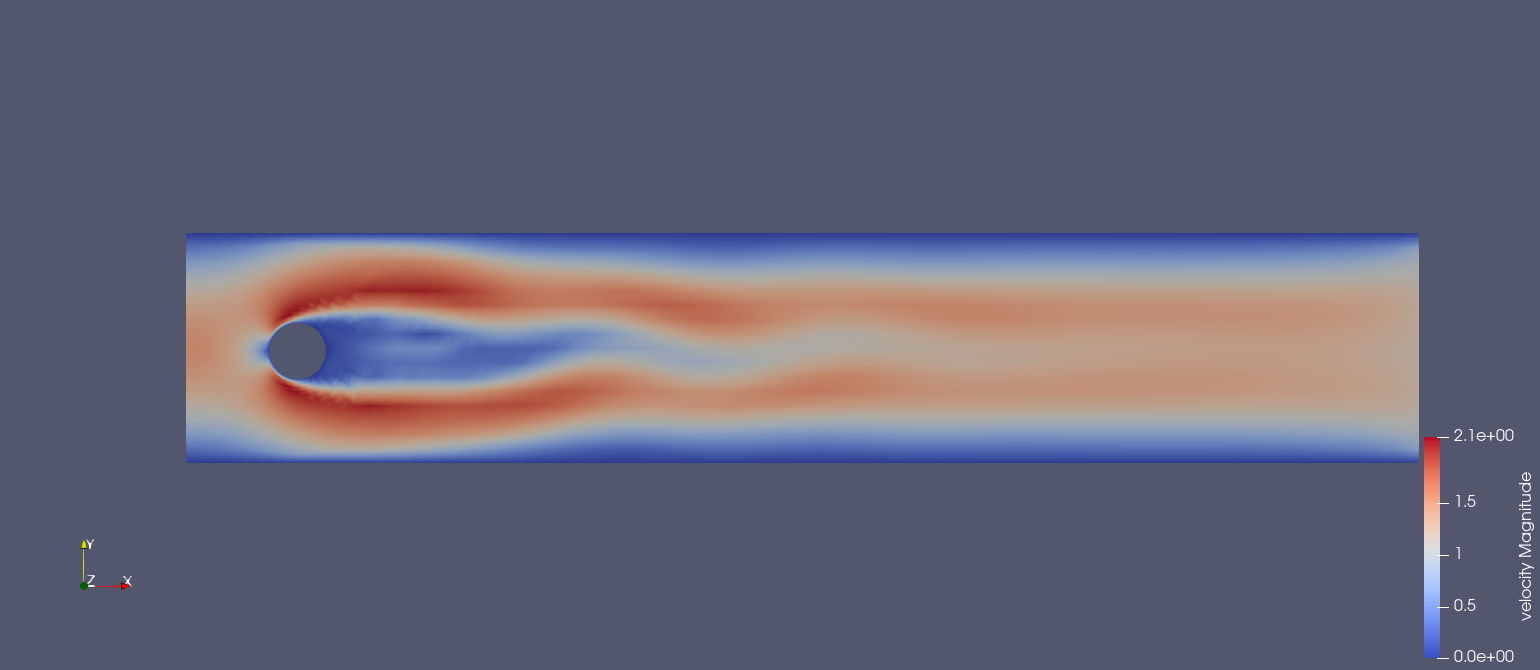
\includegraphics[scale=.2]{EMAC_time_2_5.png}
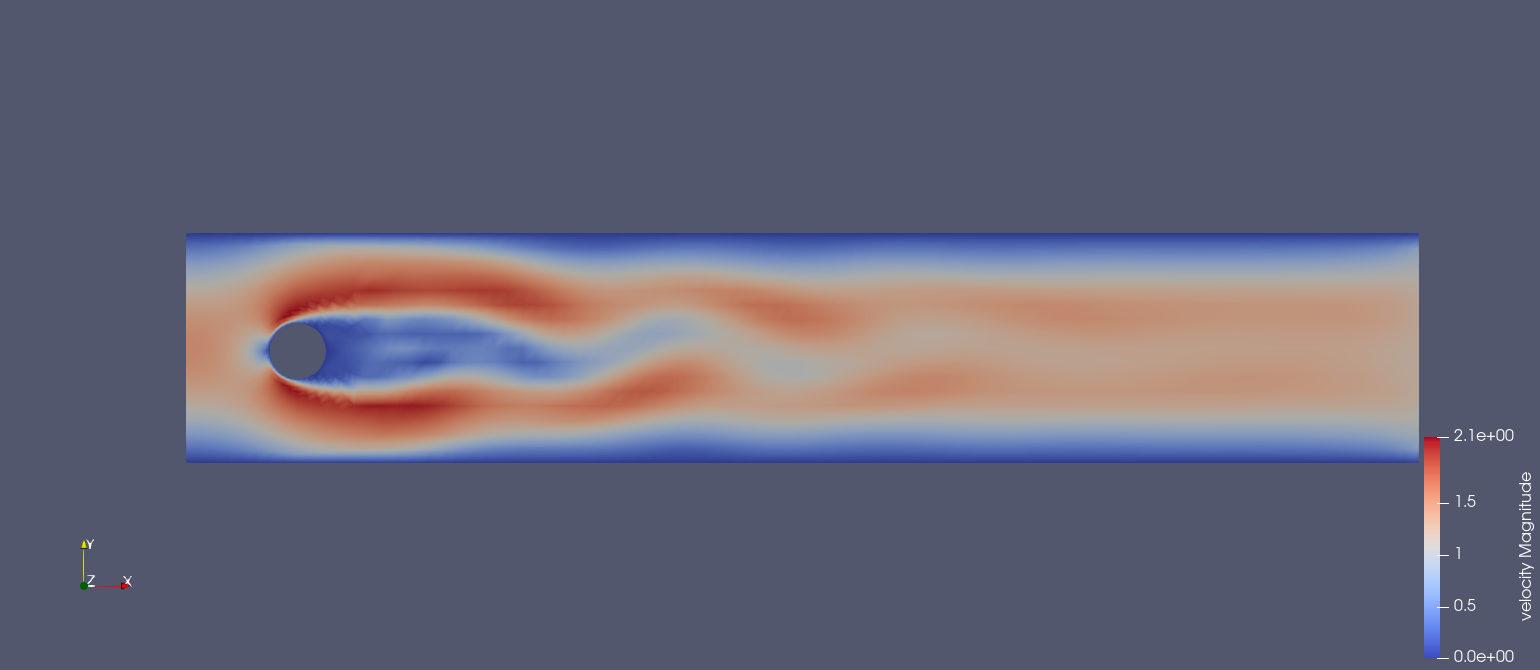
\includegraphics[scale=.2]{EMAC_time_3.png}
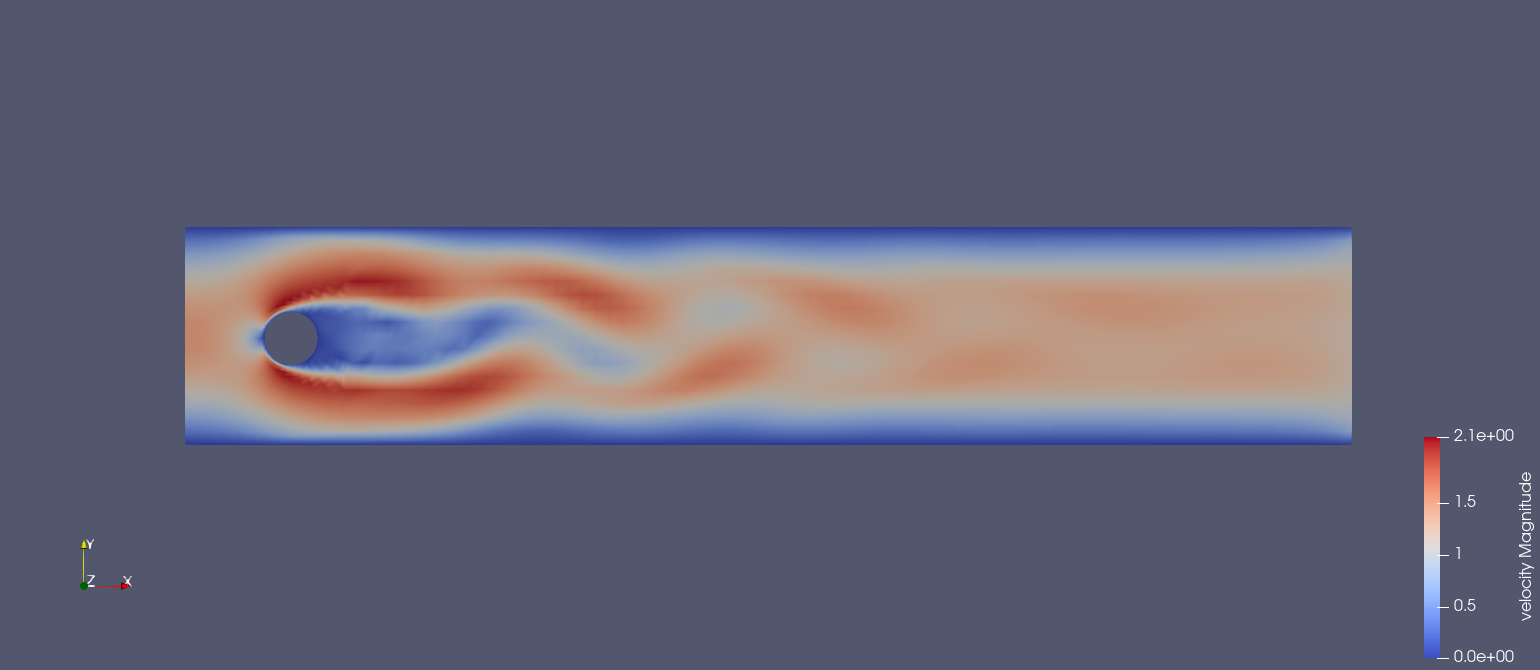
\includegraphics[scale=.2]{EMAC_time_3_5.png}
\end{figure}

\section{Conclusion}

It's very obvious here that I didn't get done all that I had hoped to.  However getting EMAC to work is pretty big.  The next obvious step is to implement EMAC-Reg and test it on coarser meshes.  From there I'd like to calculate energy, momentum and angular momentum at each timestep and confirm that EMAC-Reg is indeed doing its job properly.

In my previous work, I've only ever worked in 2d, I'd like to implement 3d problems, which shouldn't be too hard from here.  I will have to use the Palmetto cluster, but I've done that plenty before so that won't be a huge struggle.

I'd also like to change the time discretization, which is Backward Euler.  Implementing something like BDF2 or Crank-Nicolson should be an important next step.  I had to keep the time steps pretty small to get appropriate convergence here, hopefully once it changes to a higher order method we'll get better results.


\bibliographystyle{unsrt}
\bibliography{EMAC-Reg}


\end{document}